%%%%%%%%%%%%%%%%%%%%%%%%%%%%%%%%%%%%%%%%%
% University Assignment Title Page 
% LaTeX Template
% Version 1.0 (27/12/12)
%
% This template has been downloaded from:
% http://www.LaTeXTemplates.com
%
% Original author:
% WikiBooks (http://en.wikibooks.org/wiki/LaTeX/Title_Creation)
%
% License: CC BY-NC-SA 3.0 (http://creativecommons.org/licenses/by-nc-sa/3.0/)
% 
% Instructions for using this template:
% This title page is capable of being compiled as is. This is not useful for 
% including it in another document. To do this, you have two options: 
%
% 1) Copy/paste everything between \begin{document} and \end{document} 
% starting at \begin{titlepage} and paste this into another LaTeX file where you 
% want your title page.
% OR
% 2) Remove everything outside the \begin{titlepage} and \end{titlepage} and 
% move this file to the same directory as the LaTeX file you wish to add it to. 
% Then add \input{./title_page_1.tex} to your LaTeX file where you want your
% title page.
%
%%%%%%%%%%%%%%%%%%%%%%%%%%%%%%%%%%%%%%%%%
%\title{Title page with logo}
%----------------------------------------------------------------------------------------
%	PACKAGES AND OTHER DOCUMENT CONFIGURATIONS
%----------------------------------------------------------------------------------------
\PassOptionsToPackage{warn}{textcomp}
\documentclass[14pt]{extarticle}
%Paquetes para idioma español y codifcación UTF8
\usepackage[spanish]{babel}
\usepackage[utf8]{inputenc}
\usepackage{csquotes}

%%% BIBLATEX
\usepackage{biblatex}
%%% BIBLIOGRAPHY
\addbibresource{references.bib}

%fuente 'fourier'
\usepackage{fourier}
%paquete para URLs
\usepackage{url}
\usepackage[hidelinks]{hyperref}
%paquete para ubicar las imágenes
\usepackage{float}
%paquete para imágenes y en dónde las tiene que buscar
\usepackage{graphicx}
\graphicspath{{images/}}
%paquete para epígrafes
\usepackage{subcaption}
%paquete para definir los márgenes de la hoja
\usepackage[left=1.5cm,right=1.5cm,top=3cm,bottom=3cm]{geometry}
%paquete para poner todos y comentarios
\usepackage[colorinlistoftodos]{todonotes}
%paquete para trabajar con código
\usepackage{listings}
%paquete para trabajar con colores y definir propios
\usepackage{color}

%paquete para el checkmark y la cruz
\usepackage{pifont}
%paquete para el signo de copyright
\usepackage{textcomp}

%paquete para que los \texttt{} no rompan el margen de la página
\usepackage[htt]{hyphenat}

\usepackage{enumerate}
%paquete para armar layouts multicolumna
\usepackage{multicol}


%Cabeceras
\usepackage{fancyhdr}
\pagestyle{fancy}
\fancyhead[L]{Aspectos Legales y Profesionales, 2018}
\fancyhead[C]{}
\fancyhead[R]{UNPSJB}

\fancyfoot[R]{Luciano Serruya Aloisi}

%Comando para poner doble comillas más fácil
\newcommand{\dq}[1]{``#1''}
\newcommand{\cmark}{\ding{51}}
\newcommand{\xmark}{\ding{55}}

\definecolor{comment-green}{rgb}{0,0.5,0}
\definecolor{bg-light-gray}{HTML}{E9E9E9}
\definecolor{bg}{HTML}{D0B698}

\lstdefinestyle{bashstyle}{
    language=Bash,
    backgroundcolor=\color{bg},
    basicstyle=\ttfamily,
  	keywordstyle=\bfseries\color{white},
    stringstyle=\color{blue},
    commentstyle=\color{comment-green}\itshape,
    numberstyle=\color{gray},
    identifierstyle=\color{black},
    rulecolor=\color{gray},
    showstringspaces=false,
    escapeinside={\%*}{*)},
    morekeywords={},
    otherkeywords={},
    breaklines=true,
    frame=trbl, 
    framexleftmargin=25pt,
    numbers=left,
    xleftmargin=\parindent,
    frameround=tttt,
    captionpos=b,
    % re tirado de los pelos, pero es lo que hay
    % sacado de:
    % https://tex.stackexchange.com/questions/24528/having-problems-with-listings-and-utf-8-can-it-be-fixed
    inputencoding=utf8,
    extendedchars=true,
    literate={á}{{\'a}}1 {é}{{\'e}}1 {í}{{\'i}}1 {ó}{{\'o}}1 {Ó}{{\'O}}1 {ú}{{\'u}}1,
}



\begin{document}

%%%%%%%%%%%%%%%%%%%%%%%%%%%%%%%%%%%%%%%%%%%%
% En 'titlepage.tex' se encuentra la página de título
%%%%%%%%%%%%%%%%%%%%%%%%%%%%%%%%%%%%%%%%%%%%
\begin{titlepage}

    \newcommand{\HRule}{\rule{\linewidth}{0.5mm}} % Defines a new command for the horizontal lines, change thickness here

    \center % Center everything on the page
     
    %----------------------------------------------------------------------------------------
    %	HEADING SECTIONS
    %----------------------------------------------------------------------------------------

    \textsc{\LARGE UNPSJB}\\[1cm] % Name of your university/college
    \textsc{\Large Licenciatura en Sistemas OPGCPI}\\[0.5cm] % Major heading such as course name
    \textsc{\large Aspectos Legales y Profesionales}\\[0.5cm] % Minor heading such as course title

    %----------------------------------------------------------------------------------------
    %	TITLE SECTION
    %----------------------------------------------------------------------------------------

    \HRule \\[0.4cm]
    {\huge \bfseries Blockchain}\\[0.4cm] % Title of your document
    {\large \bfseries Una alternativa descentralizada para firma digital}\\[0.4cm] % Title of your document
    \HRule \\[1.5cm]
     
    %----------------------------------------------------------------------------------------
    %	AUTHOR SECTION
    %----------------------------------------------------------------------------------------


    \begin{minipage}[l]{0.5\textwidth}
        \begin{flushleft}
            \textbf{\textsf{Cátedra}}\\
            \large Dr. Guillermo Cosentino\\
            \large Lic. Bruno Damián Zappellini\\ 
            \linespread{4}
            \end{flushleft}
    \end{minipage}
    \begin{minipage}[l]{0.4\textwidth}
        \begin{flushright}
            \textbf{\textsf{Integrantes:}}\\
            \linespread{1}
            \large Luciano Serruya Aloisi\\
        \end{flushright}
    \end{minipage}\\[1.5cm]

    % If you don't want a supervisor, uncomment the two lines below and remove the section above
    %\Large \emph{Author:}\\
    %John \textsc{Smith}\\[3cm] % Your name

    %----------------------------------------------------------------------------------------
    %	DATE SECTION
    %----------------------------------------------------------------------------------------

    {\large \today}\\[1cm] % Date, change the \today to a set date if you want to be precise

    %----------------------------------------------------------------------------------------
    %	LOGO SECTION
    %----------------------------------------------------------------------------------------

    
\includegraphics[scale=1]{logoUnpsjb.png}\\[0.5cm] % Include a department/university logo - this will require the graphicx package
     
    %----------------------------------------------------------------------------------------

    % \vfill % Fill the rest of the page with whitespace

\end{titlepage}


%%%%%%%%%%%%%%%%%%%%%%%%%%%%%%%%%%%%%%%%%%%%
% INDICE
%%%%%%%%%%%%%%%%%%%%%%%%%%%%%%%%%%%%%%%%%%%%
\clearpage
\tableofcontents
\clearpage 

\lstset{style=bashstyle}

\section{Introducción}

El presente trabajo de investigación se tratará sobre la tecnología \emph{blockchain}\footnote{Infraestructura de computadoras sobre la que corre el protocolo Bitcoin, y otras criptomonedas y aplicaciones descentralizadas}, haciendo foco en sus capacidades para implementar un mecanismo de firma digital sobre la misma.

La primer parte explicará de manera amplia conceptos de criptografía y los tipos que existen, y funciones \emph{hash}. Luego, desarrollará sobre el concepto de firma digital (y la situación actual en la Argentina), y sobre la \emph{Infraestructura de Clave Pública} (\emph{PKI}).

Por último, el trabajo abarcará el concepto de \emph{blockchain} y cómo se podría implementar una infraestructura de firma digital sobre blockchain.

\subsection{Criptografía}

La criptografía es un área de estudio que consiste de varios esquemas y técnicas para transformar un mensaje en texto plano en un mensaje cifrado; este proceso de transformación se conoce como \textbf{encripción}, mientras que el proceso de conseguir el mensaje original a partir del cifrado se llama \textbf{desencripción} \autocite{StallingsCryptography}

\subsubsection{Simétrica}

La criptograía simétrica (o \emph{encripción de clave secreta}) encripta un mensaje utilizando \textbf{una única llave} - la misma llave que encripta el mensaje desencripta el mensaje cifrado para obtener de nuevo el original. 

\begin{figure}[H]
    \centering
    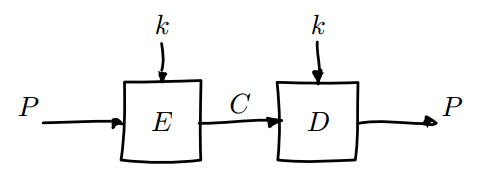
\includegraphics[width=0.8\linewidth]{images/van-houvten-simetrico.png}
    \caption*{Cifrado y descifrado simétrico (\texttt{P} representa el texto plano, \texttt{C} el mensaje cifrado, \texttt{E} y \texttt{D} las funciones de cifrado/descifrado respectivamente, y \texttt{k} la clave secreta) \autocite{VanhouvtenBlockCiphers}}
\end{figure}

Los algoritmos de encriptación simétricos pueden trabajar con \emph{bloques} (encriptando bloques de un mismo tamaño), o con \emph{flujos} (encriptando flujos de datos, pueden ser flujos de 1 bit).  

Este tipo de encriptación es muy performante y no incrementa el tamaño del mensaje, pero introduce una vulnerabilidad al tener que compartir la clave secreta entre las partes que se están queriendo comunicar.

\subsubsection{Asimétrica}

La encriptación asimétrica (o \emph{encripción de clave pública}), a diferencia de la simétrica que utiliza una única clave, necesita de dos llaves para funcionar: una \textbf{una privada} y \textbf{una pública}.  
Este sistema de encriptación se basa en que se utiliza una clave para encriptar el mensaje, y otra clave (diferente de la primera, pero relacionada) para desencriptar el mensaje. Su característica principal es que es computacionalmente inviable determinar la clave de desencripción solamente sabiendo el algoritmo de cifrado y la clave de encripción \autocite{StallingsPublicKeyPrinciples}.

Teniendo este par de claves, se puede operar de dos modos distintos:

\begin{itemize}
    \item Modo encripción: el emisor encripta el mensaje con la clave pública del receptor, de modo que sólo el receptor sea capaz que de desencriptar el mensaje (utilizando su clave privada)
    \item Modo autenticación: el emisor encripta el mensaje (o un \emph{digesto} del mensaje) con su clave privada y los anexa al mensaje. El receptor desencripta este anexo con la clave pública del emisor, y compara el anexo desencriptado con el mensaje (o el digesto pudo generar el receptor). Si son iguales, entonces se garantiza que el mensaje fue enviado por el emisor, y que no fue alterado en el camino
\end{itemize}

Claramente este tipo de encripción genera mayor seguridad en la comunicación, debido a que las claves para desencriptar los mensajes no se deben intercambiar entre las partes previamente a comenzar la comunicación (son privadas a cada cliente y no deben ser reveladas). Sin embargo, aumentan el tamaño del mensaje y no son algoritmos tan performantes como los simétricos.

\subsection{Funciones de \emph{hash}}

Otro elemento de la criptografía muy importante para blockchain son las funciones de \emph{hash} (la mayor carga de trabajo del protocolo se trata de calcular \emph{hashes}).

Las funciones \emph{hash} se tratan de funciones que toman una entrada de largo variable y lo convierten en un valor de largo fijo, también conocido como \dq{digesto} \autocite{VanhouvtenHashIntro}. Una característica muy importante de estas funciones, es que es fácil computar, pero muy difícil (hasta imposible) revertir -conseguir la entrada que originó cierto \emph{hash}-

\section{Firma digital}

El envío de un documento \emph{digitalmente firmado} es necesario cuando se precisan las siguientes tres condiciones:

\begin{enumerate}
    \item Verificar que el mensaje no fue alterado en el camino (\emph{integridad})
    \item Verificar que el emisor realmente fue el que envió el mensaje (\emph{autenticación})
    \item Verificar que el emisor quiso enviar el mensaje (\emph{no repudio})
\end{enumerate}

Para esto, la firma digital consiste en utilizar la clave privada en el \emph{modo autenticación} (como fue descripto en la subsección de \emph{Criptografía asimétrica}). 

El emisor genera un digesto del mensaje (aplicando una función de \emph{hash} al mensaje), y dicho digesto es el que se encripta con la clave privada del emisor. El resultado de encriptar el digesto se conoce como \textbf{firma digital}; se la anexa al documento y se envía. El receptor genera el mismo \emph{hash} del documento, desencripta la firma digital con la clave pública del emisor, y compara su resultado con el digesto: si son iguales, las tres condiciones anteriormente nombradas se cumplen.  

\subsection{Situación en Argentina}

El 11 de Diciembre de 2001, el Senado y la Cámara de Diputados de la Nación Argentina sancionó con fuerza de ley la \emph{Ley de Firma Digital} (Ley 25506). En su primer capítulo, en el artículo 2, se describe a la firma digital de la siguiente manera \autocite{LeyFirmaDigitalCapUno}:

\begin{quote}\itshape
Se entiende por firma digital al resultado de aplicar a un documento digital un procedimiento matemático que requiere información de exclusivo conocimiento del firmante, encontrándose ésta bajo su absoluto control. La firma digital debe ser susceptible de verificación por terceras partes, tal que dicha verificación simultáneamente permita identificar al firmante y detectar cualquier alteración del documento digital posterior a su firma
\end{quote}

Esta definición da a entender un procedimiento de firma digital similar al descripto previamente, donde el emisor firmaría con su \emph{clave privada} (\emph{conocimiento encontrado bajo absoluto control del firmante}) el mensaje o su digesto.

A lo largo del desarrollo de la ley, se habla también de conceptos relacionados con la tecnología \emph{PKI}, tales como \emph{Certificado}, \emph{Certificador licenciado}, y \emph{Ente licenciante}.    

\section{\emph{PKI}: \emph{Public Key Infrastructure}}
La RFC 4949 define la \emph{Infraestructura de Clave Pública} (\emph{PKI}) como un conjunto de hardware, software, personas, políticas, y procedimientos necesarios para crear, manejar, almacenar, distribuir, y remover certificados digitales basados en criptografía asimétrica. El objetio principal para desarrollar PKI es establecer una forma segura, conveniente, y eficiente de adquirir claves públicas \autocite{StallingsPKI}.

PKI se compone de varios componentes:

\begin{itemize}
    \item Entidad final: concepto que engloba tanto usuarios finales, dispositivos o servidores, o cualquier otra entidad que necesite ser identificada en el ámbito de certificados de clave pública. Estas entidades mayormente consumen y/o soportan servicios relacionados con PKI
    \item Autoridad de Certificación (\emph{Certification Authority - CA}): emisor de certificados y, usualmente, de las listas de revocación de certificados
    \item Autoridad de Registro (\emph{Registration Authority - RA}): componente opcional (la CA puede llevar a cabo sus funciones) que se encarga de verificar que un usuario que solicita un certificado es quién dice ser.
    \item Emisor de CRL: componente opcional (la CA puede llevar a cabo sus funciones) que se encarga de emitir las \emph{listas de revocación de certificados} (listas que indican todos los certificados que han sido revocados, y por lo tanto no se deberían aceptar)
    \item Repositorio: termino genérico para representar cualquier método para almacenar certificados y listas de revocación de certificados para que puedan ser accedidos por usuarios finales
\end{itemize}

\subsection{Funcionamiento de \emph{PKI}}

Cuando un cliente desea obtener un certificado de una CA, primero debe demostrar que es quién dice ser. En el caso de un servidor web, esta verificación de identidad podría consistir en demostrar que el dominio para el cual desea obtener el certificado realmente le corresponde. Estos pasos iniciales son llevados a cabo contra la RA (o la propia CA, en caso de que no haya RA).

Una vez demostrado que el servidor es quién dice ser, el cliente le debe enviar su clave pública a la CA; este último generará un certificado (con una fecha de vencimiento) en el cual incluye el nombre de dominio, la clave pública del servidor, y la firma digital de la CA (provee autenticidad de que la CA confía en el servidor). Teniendo este certificado, usuario finales se podrán conectar de manera segura con el servidor web.

Ahora bien, la CA que emitió el certificado para el servidor a su vez también cuenta con un certificado, el cual fue emitido por otra CA. Las \textbf{CA raíz} (\textbf{\emph{root CA}}) son los primeros emisores de esta cadena de certificados. Los navegadores web ya cuentan con las claves públicas de varias CA raíz para validar los certificados. 

Cuando un usuario se conecta al servidor, primero le solicita el certificado al servidor; éste le contesta enviándole tanto su certificado como el de su CA. Primero el cliente verifica el certificado de la CA validando la firma digital con la clave pública de la CA raíz que emitió el certificado (el navegador cuenta con dicha clave pública). Luego, repite el proceso con el certificado del servidor, y con la clave pública de la CA intermedia.

\begin{figure}[H]
    \centering
    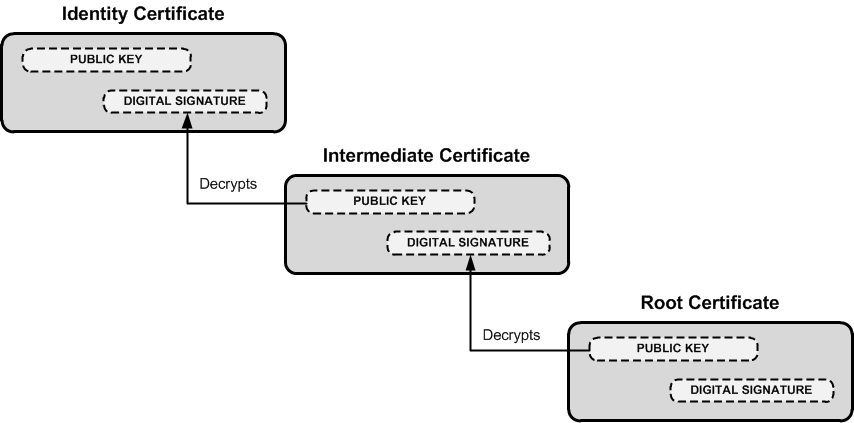
\includegraphics[width=0.8\linewidth]{images/pki-chain-of-trust.png}
    \caption*{\emph{Verificación en cadena} de certificados \autocite{FirenetPKIChainOfTrust}}
\end{figure}

Una vez verificados todos los certificados, se puede establecer una conexión segura entre el cliente y el servidor.

\section{\emph{Blockchain}}

Blockchain, o la \emph{cadena de bloques}, es el \dq{libro de cuentas} público, ordenado en el tiempo, e \emph{inmutable} de todas las transacciones en la redes de criptomonedas. Cada bloque está identificado por un \emph{hash} en la cadena y está vinculado con su bloque anterior referenciando su \emph{hash}. Todos los bloques están relacionados con su bloque anterior, a excepción del primer bloque, también llamado bloque \emph{génesis}. También se puede definir blockchain como una base de datos distribuida, en donde cada nodo tiene una copia entera de la base.

Bloques nuevo son añadidos a la cadena cada cierto tiempo. El protocolo de blockchain maneja una \emph{dificultad}\footnote{La dificultad signifca qué tan difícil es para los mineros generar un bloque nuevo} para agregar nuevos bloques. Puede ir aumentando o disminuyendo según la capacidad de cómputo disponible en la red, para que se mantenga la frecuencia de un bloque nuevo cada el tiempo determinado (10 minutos en la blockchain de Bitcoin) \autocite{MasteringBlockchainBlockchain}.

\subsection{Minería de bloques}

La minería de un bloques es una tarea que conlleva muchos recursos (de hardware y de electricidad) mediante el cual se agregan nuevos bloques a la red. Los bloques contienen las transacciones que son validadas mediante el proceso de minado (llevado a cabo por los nodos mineros). 

Los \emph{mineros} (computadoras que están corriendo el software necesario para ejecutar los algoritmos de minado) que generen correctamente el nuevo bloque, se llevan una recompensa (en Bitcoin, el minero se lleva una cantidad de bitcoins). De esta forma, existe un incentivo para que se dispongan computadoras y recursos en pos de que funcione el protocolo y de mantenerlo activo.

Cuando se genera un nuevo bloque, el minero que lo generó hace una \emph{difusión} del bloque nuevo a toda la red para que el resto de los mineros lo verifique. Esto asegura el sistema contra fraudes y ataques de \emph{doble gasto}\footnote{Situación en la que se realizan dos o más transacciones con un mismo dinero}. 

El concepto de \dq{minería} se debe a que las monedas (en el caso de las blockchain de criptomonedas) se crean o se \dq{emiten} al crear un nuevo bloque; es una analogía a la minería de oro, en donde en base a un trabajo se obtiene algo de valor.

\subsection{Prueba de trabajo}

La prueba de trabajo (\emph{Proof of Work}) es una demostración de que suficiente poder computacional fue empleado para construir un bloque válido. En este modelo, los nodos compiten para ser seleccionados en proporción a su capacidad computacional.

La prueba de trabajo consiste en calcular el \emph{hash} del bloque. Éste se compone de la suma de todos los datos del bloque, y debe comenzar con \emph{n} número de ceros (o que sea menor a cierto valor). La cantidad de ceros o el valor \emph{objetivo} está definido por la \emph{dificultad} de la red.     

Debido a que es fácil calcular el \emph{hash} de un valor, pero imposible conseguir el valor original a partir de un \emph{hash}, la única forma de calcular el \emph{hash} del bloque es \textbf{con fuerza bruta} (probar valores hasta encontrar un resultado). El campo \texttt{nonce} de la cabecera del bloque es el que tienen que ir incrementando los mineros hasta encontrar el \emph{hash} indicado.

\begin{figure}[H]
    \centering
    \[ H(N || P\_hash|| Tx_1 || Tx_2 || ... || Tx_n) < Objetivo \]
    \caption*{Cálculo de la cabecera del bloque, donde \texttt{H} es la función de \emph{hash}, \texttt{N} es el \emph{nonce}, \texttt{P\_hash} es el \emph{hash} del bloque anterior, \texttt{Tx} son las transacciones que incluye el bloque, y \texttt{Objetivo} la dificultad}
\end{figure}

Una vez conseguido el \emph{hash}, el bloque es inmediatamente difundido por la red. Debe ser aceptado por los otros mineros para ser agregado a la red \autocite{MasteringBlockchainProofOfWork}. 

Blockchain se dice que es \dq{inmutable} debido a la dificultad que conllevaría modificar un bloque. En caso de modificar un bloque, el \emph{hash} se vería modificado también, por lo tanto habría que recalcularlo (lo cual es una tarea muy costosa). No solo eso, sino que si el bloque no es el último de la cadena -tiene otros bloques por delante-, habría que modificar esos otros bloques también (ya que cada bloque tiene el \emph{hash} del anterior, a modo de puntero). Por lo tanto, blockchain no es en sí inmutable, pero modificar un dato que ya se escribió en un bloque conllevaría demasiado trabajo, haciéndolo inviable.

\subsubsection*{Algoritmo de minado}

La secuencia de pasos que llevan a cabo los mineros que crear un nuevo bloque es la siguiente \autocite{MasteringBlockchainMiningAlgorithm}

\begin{itemize}
    \item El bloque anterior se recupera de la red
    \item Se obtiene un conjunto de posibles transacciones que podrían conformar el bloque
    \item Computar el \emph{hash} de la cabecera del bloque con un \emph{nonce} = 0 
    \item Si el \emph{hash} obtenido es menor al objetivo, detener el proceso
    \item Si no es menor, repetir el proceso incrementando el \emph{nonce} 
\end{itemize}

\subsection{\emph{PKI} sobre \emph{Blockchain}}
La Infraestructura de Clave Publica provee un metodo seguro para autenticar identidades sobre Internet. Define las políticas y los procedimientos necesarios para emitir, gestionar, validar y distribuir certificados para poder usar encripción asimétrica de forma segura. El manejo de claves públicas de PKI usualmente está basado en el estándar de certificados \emph{X.509}, que provee verificación de posesión de una clave privada gracias a un ente externo (Autoridad Certificante).

Sin embargo, las CA no dejan de ser \emph{puntos únicos de fallo} (\emph{single point of failure}), lo que significa que errores presentes (principalmente de seguridad, haciendo propenso a una CA al ataque de un \emph{hacker}) en las CA significan emisiones de certificados sin autorizar \autocite{PKICAErrors}. Estos problemas no sólo afectan a las CA intermedias, sino que a las raíces también.

Para resolver este problema, se plantearon dos soluciones distintas. La primera de ellas consiste en una \emph{Infraestructura de Clave Pública basada en logs} (\emph{log-based PKI}), la cual consiste en implementar servidor con alta disponibilidad que registren y monitoreen todos los certificados emitidos por la CA. Los certificados no son considerados válidos hasta no ser registrados en el \emph{log}, de esta manera se expone rápidamente cualquier emisión incorrecta. Ante la detección de cualquier comportamiento extraño por parte de la CA, es responsabilidad del dominio de actuar frente a los certificados no autorizados que han sido emitidos.

La otra solución planteada es un enfoque descentralizado: \emph{Red de Confianza} (\emph{Web of Trust}). En esta propuesta, los usuarios son encargados de indicar que otros usuarios son confiables firmando sus certificados. De esta forma, un usuario acumula varias firmas en su certificado, generando confianza (enfoque similar al de PGP). De esta forma se elimina el punto único de fallo, pero la desventaja que se introduce es que los nuevos usuarios que ingresen a la red no tendrán ninguna firma en su certificado, por lo tanto les resultará inútil.

En el contexto de PKI, blockchain puede proveer características de seguridad muy valiosas como revocación de certificados, eliminación de puntos de fallo, y un registro de transacciones fiable.

Existen varias implementaciones de PKI sobre blockchain; \autocite{BlockchainBasedPKIFramework} plantea un \emph{framework} gestionar un sistema de PKI sobre blockchain que soporta la revocación de certificados. Su diseño está basado en \emph{certificados X.509 híbridos}.

\begin{figure}[H]
    \centering
    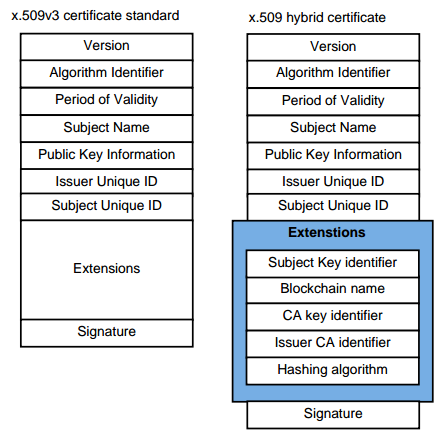
\includegraphics[width=0.8\linewidth]{images/blockchain-pki-certificates.png}
    \caption*{Certificados X.509 híbridos \autocite{BlockchainBasedPKIFramework}}
\end{figure}

La idea principal de esta implementación es que cada CA tiene un \emph{contrato inteligente} (\emph{smart contract})\footnote{Programas que corren sobre la blockchain y modifican su estado \autocite{SmartContracts}} dedicado que incluye la siguiente información:

\begin{itemize}
    \item Lista on los \emph{hashes} de los certificados emitidos
    \item Lista con los \emph{hashes} de los certificados revocados
\end{itemize}

Tanto los CA raíces como los CA intermedios se representan con un contrato dedicado. Con esta estructura, crear una nueva CA consiste en crear un nuevo contrato (la CA padre crea el contrato, y agrega el \emph{hash} del certificado de la CA hija a su lista de CA emitidos).

Como todos los nodos que componen la red tienen una copia de la base de datos (tienen una copia de la blockchain), verificar un certificado sigue siendo el mismo procedimiento que en la versión original de PKI - se debe validar toda la cadena de certificados, desde la CA raíz hasta el usuario final.

En el caso de que se deba revocar un certificado, sencillamente la CA encargada de emitir dicho certificado actualiza sus listas de \emph{hashes} moviendo el \emph{hash} del certificado a revocar de la lista de \emph{hashes} emitidos a la de los revocados. Esta notificación será enviada al resto de los nodos instantáneamente, logrando una actualización de los certificados activos, y eliminando la necesidad de una CRL. 

Esta característica también significa una protección frente a \emph{atanque de hombre en el medio} (\emph{Men-in-the-middle attacks})\footnote{Ataque a la seguridad que consiste en enviar un certificado falso, haciéndolo pasar por uno válido, para así interceptar la comunicación}. En la versión original de PKI, en caso de que una CA se vea comprometida, los usuarios finales tendrían que esperar a la actualización de la CRL para recién anular el certificado de la CA en cuestión (mientras tanto podrían recibir certificados falsos firmados por la CA comprometida). Con PKI corriendo sobre blockchain, esta situación se vuelve virtualmente imposible. 

\section{Conclusión}

Blockchain como tecnología moderna, sigue en una etapa de mucho auge. Debido a esto, muchas soluciones de software o arquitecturas se intentan plantear en blockchain, muchas sin éxito.

Particularmente con PKI, blockchain (complimentado también con los \emph{smart contracts}) puede ser una buena alternativa, logrando tener una infraestructura que certifica la autenticidad de un ente, corriendo en una red descentralizada de computadoras sin contar con un esquema de confianza, manteniendo la seguridad y la integridad, y sin contar con un administrador central \autocite{SmartContractsUseCases}.



%%%%%%%%%%%%%%%%%%%%%%%%%%%%%%%%%%%%%%%%%%%%
% FIN DOCUMENTO, AHORA REFERENCIAS
%%%%%%%%%%%%%%%%%%%%%%%%%%%%%%%%%%%%%%%%%%%%
\clearpage
\printbibliography

\end{document}
